\subsection{Design two}
Compared to several of the vehicle-game controllers available, this design-idea obviates controlling the vehicle using a steering-wheel-like controller. In this design, the user grabs hold of two blocks and moves these around on a flat surface e.g. a table, and thus controlling the behaviour of the car.

\subsubsection*{Description}

\begin{figure}[h]
\centering
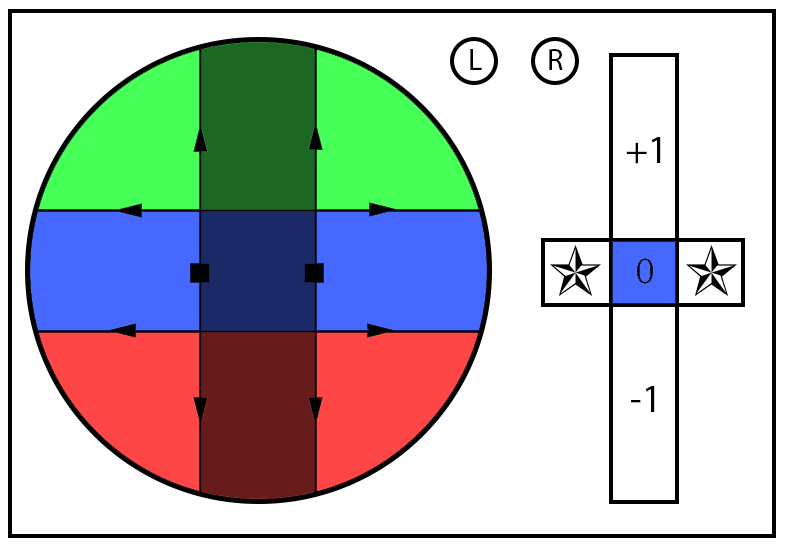
\includegraphics[scale=.75]{Design21}
\caption{Playing area.}
\label{fig:design21}
\end{figure}

What the user need in order to be able to control the car using this design is two blocks of different colours that can be held without covering the top of the block. Next, the user needs a webcam, which will be placed over the area in which the user is moving the blocks around in looking down to see the top face of the blocks. Ideally the user would also have a piece of paper, with the “playing area” drawn onto it. It is assessed that the optimal size is A3 as to avoid expansive gestures, which would be the result of a too big “playing area”. Conversely, a too small “playing area” could cause misreading and misplacements.
\bigskip

The “playing area” is illustrated on figure \ref{fig:design21}, where on the left side a circle is drawn. The user will move one of the blocks around in this circle and the car will accelerate when the block is in the green areas, decelerate when in the red areas and neutral when in the blue areas. By moving the block to the left or right, i.e. moving the block inside one of the bright-coloured areas, the car will turn accordingly while still accelerating, decelerating or none of those.

The other block used in this controller, is used to change the gear up and down and to activate additional features (currently this design supports two additional features). The shape on the left side of figure \ref{fig:design21} is where this other block is used. When the user is not changing gear or activating another feature, the block is to be placed inside the blue tile containing the number “0”. If the user will move the block up or down to change gear accordingly into the tiles tagged ‘+1’ for increase gear, and ‘-1’ for decreased gear. To activate one of the additional features, the user will move the block either left or right from the blue tile and into the tiles with the stars, which will then activate the feature set to the respective tile.

In the top of figure \ref{fig:design21} there are two circles marked “L” and “R”. Each of the two blocks will be placed in one of the two circles before the controller will be active. This means that the controller has to determine the block that is used to turn and accelerate/decelerate the car, which will be placed in “L”, while the block placed in “R” will be used to change gear and activate additional features.

Though the user does not need the playing area to be drawn on something in order to use the controller, it would be easier for the user to keep track of what control he/she is activating, when the tiles are illustrated beneath the blocks. However, the colours used in figure \ref{fig:design21} are not mandatory, but simply used in order to facilitate the concept-description.

\subsubsection*{How does this design fulfil the design requirements? (IGNORE TEMPORARILY)}

\subsubsection*{Pros and cons}
Pros:
\begin{itemize}
\item The controller is very different from other controllers which might arouse curiosity.
\item Only a computer and a webcam needs to be bought, other materials can be home-made.
\item Is usable for several racing games (or alike).
\item Can be expanded to support several additional features (e.g. up/down gear-shift could be replaced) or additional tiles could be added.
\end{itemize}
Cons:
\begin{itemize}
\item Could be difficult to place the blocks on the tiles precisely while maintaining the focus in the game.
\item With the current setup, the user needs the computer and webcam to be separated, thus eliminating the use of a laptop with its webcam.
\end{itemize}

\subsubsection*{Image Processing.. how?}
In order to detect how the user is moving around the blocks, colour recognition would be an easy way to distinguish between the two blocks. The two blocks could be separated as two BLOBs and according to each BLOB’s position in the frame, captured by the webcam, relative to the tiles in the playing area, the user’s intention could be registered. This however, would require the blocks to be of easily distinguishable colours that does not blend-in with each other or the colours in the background.